%% Based on http://tex.stackexchange.com/questions/150900/latex-coding-for-statement-of-purpose

\documentclass{article}

\usepackage[
  a4paper,
  margin=1in,
  headsep=4pt % separation between header rule and text
]{geometry}

\usepackage{xcolor}
\usepackage{fancyhdr}
\usepackage{tgschola}
\usepackage{lastpage}
\usepackage{graphicx}   % figures
\usepackage{amsmath}    % math
\usepackage[round]{natbib} % citations: \citep, \citet
\usepackage{hyperref}   % links
\usepackage{enumitem}   % compact lists
\usepackage{wrapfig}
\setlength{\intextsep}{6pt plus 2pt minus 2pt} % space above/below in-text floats
\setlength{\columnsep}{12pt}                   % gap between text and figure


% ---------- Header / Footer ----------
\newcommand{\soptitle}{Research Statement}
\newcommand{\yourname}{Wassim Kabalan}
\newcommand{\youremail}{wassim@apc.in2p3.fr}
\newcommand{\yourweb}{https://askabalan.github.io}
\newcommand{\wk}[1]{\textcolor{red}{#1}}

\pagestyle{fancy}
\fancyhf{}
\renewcommand{\headrulewidth}{0.4pt}
\renewcommand{\footrulewidth}{0pt}
\fancyhead[C]{%
  \footnotesize\sffamily
  \yourname\quad
  web: \textcolor{blue}{\itshape\yourweb}\quad
  \textcolor{blue}{\youremail}}
\fancyfoot[C]{\footnotesize Page \thepage\ of \pageref{LastPage}}

% ---------- Statement section marker (optional) ----------
\newcommand{\statement}[1]{\par\medskip\noindent\textcolor{blue}{\textbf{#1:}}\ }

% ---------- Link & PDF metadata ----------
\hypersetup{
  colorlinks=true,
  urlcolor=blue,
  linkcolor=blue,
  citecolor=blue,
  pdftitle={\yourname - \soptitle},
  pdfauthor={\yourname}
}

% ---------- Lists a bit tighter ----------
\setlist[itemize]{noitemsep,topsep=2pt,leftmargin=*,parsep=0pt,partopsep=0pt}

\begin{document}

\begin{center}
  {\LARGE \soptitle}\\[4pt]
  {\large of \yourname}
\end{center}

\hrule
\vspace{1pt}
\hrule height 1pt
\bigskip

% =========================
% Introduction
% =========================
\section*{Introduction}
I am a PhD candidate in computational cosmology at the AstroParticule et Cosmologie (APC, CNRS/IN2P3) in Paris. My work sits at the interface of CMB analysis and large-scale structure (LSS), where I build open-source, Python/JAX pipelines that are both differentiable and distributed for next-generation surveys. On the CMB side, I develop a spatially varying parametric component-separation method (via FURAX) to reduce bias in the tensor-to-scalar ratio \(r\) for Simons Observatory– and LiteBIRD–like data. On the LSS side, I lead \textbf{jaxDecomp} (multi-GPU 3D domain decomposition + distributed FFTs) and contribute to \textbf{JaxPM} (differentiable particle–mesh dynamics) to enable gradient-based weak-lensing inference at LSST scale. I am a member of the LSST Dark Energy Science Collaboration (DESC) and the Simons Observatory collaboration, and I prioritize reproducible, survey-ready software that runs from laptops to supercomputers and supports end-to-end uncertainty propagation.

% =========================
% CMB
% =========================
\section*{CMB: Spatially Varying Component Separation}
Primordial B-modes provide a decisive test of inflation and are summarized by the tensor-to-scalar ratio \(r\) \citep{Kamionkowski2016}. Constraints are increasingly limited by spatially varying Galactic foregrounds rather than instrument noise: dust and synchrotron spectra change across the sky; enforcing constant spectral parameters leaks power into large-scale B-modes and biases \(r\) \citep{Planck2018IV}.

This spatial variability challenges even modern parametric component-separation frameworks: assumptions of sky-constant (or coarse-region) spectral parameters can lead to leakage and bias when SEDs drift across the sky \citep{Planck2018IV,FGBusterASCL}. This motivates a spatially varying, parametric approach that is computationally tractable at survey scale and remains differentiable end-to-end, so we can search over many partitions and propagate uncertainties.

I built a JAX-native component-separation pipeline by contributing to \textbf{FURAX}\wk{[WHAT TO CITE]} within the SciPol project\footnote{SciPol Project: \url{https://github.com/CMBSciPol}}. Foreground spectral parameters are modeled as spatially varying fields; we assign clustered, per-patch \((\beta_d, T_d, \beta_s)\) and fit them jointly across frequencies using GPU-accelerated L-BFGS from \textbf{Optax} \citep{Optax} in \textbf{JAX} \citep{Bradbury2018JAX}. Per-patch parameters are applied to pixels via mask-aware, vectorized JAX indexing on HEALPix maps, keeping the full path from parameters to cleaned CMB maps end-to-end differentiable. To capture spatial variation robustly, I generate candidate spherical clusterings on HEALPix~\citep{Gorski2005,healpy} grids with \textbf{jax-healpy}~\citep{jax-healpy} and run a vectorized sweep using \textbf{jax-grid-search}~\citep{jax-grid-search} to evaluate many clusterings, noise realizations, and sky regions in parallel—batched/sharded across GPUs so the procedure remains inside JAX and reproducible. I then select the partition that minimizes the variance of the cleaned CMB under the mask.

FURAX follows and modernizes the parametric component-separation approach of \textbf{FGBuster}, replacing its core with a \textbf{JAX} backend; on identical configurations at moderate $n_{\rm side}$, we measure up to $\sim$200$\times$ speedups \citep{FGBusterASCL}.

\begin{wrapfigure}[12]{r}{0.47\textwidth} % try 8–14 until it fits
  \vspace{-25pt}
  \centering
  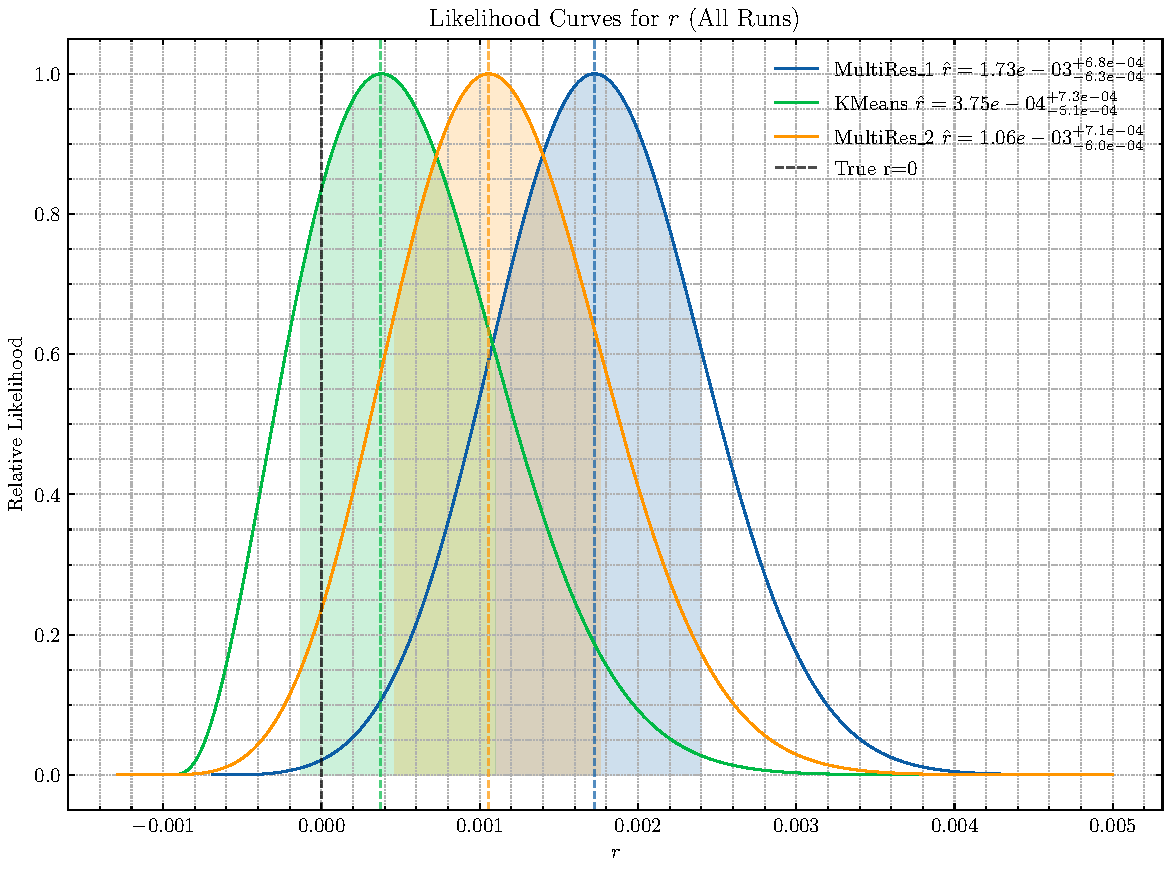
\includegraphics[width=\linewidth]{figs/r_likelihood_distribution.pdf}
  \caption{Posteriors for $r$ across partitionings. The selected spherical clustering shifts $\hat r$ toward the injected value and lowers low-$\ell$ residuals.}\label{fig:rposterior}
\end{wrapfigure}



On Simons Observatory– and LiteBIRD–like simulations \citep{SO2019,LiteBIRD2019} constructed with \textbf{PySM} (\texttt{c1d1s1}, spatially varying SEDs) \citep{PySM}, the data-selected partition lowers residual \(C_\ell^{BB}\) at low \(\ell\) and moves \(\hat r\) toward the injected value relative to uniform-parameter or fixed multi-\(n_{\text{side}}\) schemes. As seen in Fig.~\ref{fig:rposterior} (right), the posterior \(p(r\mid\text{data})\) centers nearer \(r_{\rm true}\) with comparable or tighter 68\% intervals.

\newpage

% =========================
% LSS
% =========================
\section*{LSS: Map-level Inference with Differentiable, Distributed Particle–Mesh}
Weak gravitational lensing encodes the projected matter distribution in shear/convergence maps. At LSST depth and area the signal is markedly non-Gaussian, and survey realism (masking, variable depth, PSF) breaks many assumptions behind two-point, harmonic-space analyses; a simulation-based inference (SBI) / forward-modeling approach retains information beyond the power spectrum and propagates systematics consistently from parameters to maps and back \citep{Cranmer2020SBI}. In this setting we target the joint posterior
\[
p(\theta, z \mid x)\ \propto\ p(x\mid \theta, z)\,p(z\mid \theta)\,p(\theta),
\]
over cosmological parameters \(\theta\) and latent fields \(z\) (e.g., the initial density), using the maps themselves as the data vector. Making this practical at survey volume requires a forward model that is both distributed and differentiable so gradients can drive HMC/NUTS or variational methods.

I evaluate \(p(x\mid\theta,z)\) with a fast Particle–Mesh (PM) \(N\)-body scheme, where gravity is solved on a mesh via Poisson’s equation and particles are advanced with a symplectic kick–drift–kick integrator; exchange between particles and mesh uses Cloud-in-Cell (CIC) assignment/interpolation \citep{HockneyEastwood1988}. Implemented inside \textbf{JAX}, PM\,+\,CIC becomes end-to-end differentiable, so gradients flow from map-level objectives back to initial conditions and cosmological parameters \citep{Bradbury2018JAX}.

Upcoming wide-field surveys (LSST, Euclid) will map a large fraction of the sky at high depth. To translate these data into tight cosmological constraints, forward models must combine survey-scale volumes (to capture long-wavelength modes and realistic systematics) with high spatial and mass resolution (to resolve non-linear structure formation and small-scale effects). Meeting both demands requires simulators that are fast, distributed across accelerators, and differentiable, so that gradients can drive simulation-based inference and propagate uncertainties end-to-end.

My contribution. I developed \textbf{jaxDecomp}~\citep{jaxDecomp}, an open-source JAX library for multi-GPU 3D domain decomposition and distributed FFTs using \textbf{NCCL} collectives with halo exchange \citep{NCCL}. Its primitives are \verb|jit/pjit/grad|-compatible, so Poisson solves and stencil forces remain inside autodiff even when sharded across accelerators. I integrated these capabilities into \textbf{JaxPM} \wk{WHAT TO CITE}, adding differentiable PM time-stepping, CIC paint/read, and distributed \(k\)-space solves—yielding a fully distributed, end-to-end differentiable PM engine in JAX \citep{Bradbury2018JAX}. On Jean Zay I demonstrated survey-volume PM evolution on 32 GPUs with gradients intact (Fig.~\ref{fig:lss-two}, left). The resulting stack (\textbf{jaxDecomp} + \textbf{JaxPM}) plugs directly into \textbf{NumPyro}/\textbf{BlackJAX} for gradient-based map-level inference at LSST scale \citep{NumPyro,BlackJAX}.

Born lensing and spherical projection. After the \(N\)-body evolution, I produce shear/convergence maps with a Born-approximation lensing pipeline in \textbf{JaxPM}, integrating the density along the line of sight to obtain \(\kappa\) (and \(\gamma\) when needed). Convergence maps derived for LSST will exceed \(\sim 10^\circ\) on a side; at this size the flat-sky approximation becomes inaccurate, so the projection is performed on the sphere. The spherical painting is implemented in \textbf{JaxPM} and is based on HEALPix/\texttt{healpy} functionalities that I developed and integrated in \textbf{jax-healpy} \citep{Gorski2005,healpy,jax-healpy}. The full chain—PM \(\rightarrow\) spherical projection \(\rightarrow\) Born lensing—stays inside \textbf{JAX}, scales across GPUs, and is differentiable. For validation, I compared JaxPM–Born \(\kappa\) power spectra to the \textbf{DORIAN} pipeline on identical boxes and source planes; across \(z_s=\{0.3,0.5,0.8\}\) the agreement is \(\approx 2\%\) over the measured \(\ell\) range \citep{DORIAN}.

% =========================
% Combined two-panel figure (one per project)
% =========================
\begin{figure}[!t]
  \centering
  \begin{minipage}[t]{0.49\linewidth}
    \centering
    \includegraphics[width=\linewidth]{figs/kappa_power_vs_dorian.pdf}
  \end{minipage}\hfill
  \begin{minipage}[t]{0.49\linewidth}
    \centering
    \includegraphics[width=\linewidth]{figs/nbody_jeanzay_32gpu.png}
  \end{minipage}
  \caption{Left: $\kappa$ power spectra—JaxPM (Born) vs \textsc{dorian} on identical
  boxes/source planes across $z_s=\{0.3,0.5,0.8\}$; $\sim$2\% agreement over the measured
  $\ell$ range. Right: 32-GPU N-body on Jean Zay with JaxPM\,+\,jaxDecomp
  (initial field $\rightarrow$ LPT $\rightarrow$ non-linear evolution), demonstrating
  survey-volume evolution with gradients preserved.}
  \label{fig:lss-two}
\end{figure}

% =========================
% Synergy
% =========================
\section*{Synergy with CCA and the Flatiron Institute}
CCA’s mission to advance reproducible, open computational methods is a natural fit for my work. I aim to continue producing rigorously reproducible research—open, tested, and well-documented releases with CI’d benchmarks, containers, and clear provenance—and to contribute across a stack of open-source packages that take us from simulations to cosmological answers: \textbf{FURAX} (JAX-based toolkit for differentiable algebraic computation), \textbf{jaxDecomp} (multi-GPU domain decomposition and distributed FFTs), \textbf{JaxPM} (differentiable PM and Born lensing), and \textbf{jax-healpy} utilities. I will also lead performance and scalability efforts on Flatiron hardware to responsibly push software and hardware limits, informing design and ensuring portability across CPU/GPU backends. Building on my experience teaching and giving tutorials, I plan to expand workshops and training, mentor students, and contribute to internal onboarding and documentation. As an active member of SO and DESC, I will maintain these collaborations and keep expanding my network at CCA, contributing to cross-survey, cross-probe efforts and helping cycle methods back into robust community releases under Flatiron/CCA stewardship.


% =========================
% Future Work
% =========================
\section*{Future Work: LSST-Scale Application and Baryonification}
My near-term goal is to move from validated simulations to \emph{real LSST data}. I will build an end-to-end, map-level inference pipeline that ingests shear/convergence maps with realistic survey features (masking, variable depth, PSF and shear calibration, tomographic \(n(z)\) uncertainties). The forward model already supports spherical projection and Born lensing; extending this to survey footprints and selection will enable tile-wise HMC/NUTS (NumPyro/BlackJAX) over the LSST footprint while preserving autodiff and reproducibility. Particular attention will go to uncertainty propagation (noise, calibration, and photo-$z$) so that posterior credible regions reflect survey systematics, not just statistical noise.

I will \emph{augment the forward model with a differentiable, physically motivated baryonification module} integrated into \textbf{JaxPM}. Beyond empirical prescriptions \citep{Schneider2015Baryonification}, I plan to incorporate a recent, physically grounded, differentiable approach \citep{PhysBaryon2025} that ties parameters to gas thermodynamics and feedback. The module will operate on lightcone shells/fields, expose interpretable parameters (e.g., gas fractions, ejection radii, stellar components), and remain compatible with JAX autodiff so gradients flow from LSST objectives back to both cosmology and baryonic parameters. Calibration will proceed against hydrodynamical benchmarks and summary-statistic targets (power spectrum and beyond), with explicit checks that the added expressivity improves small-scale fits without biasing large scales.

Finally, I aim to \emph{inform baryonification with CMB-based priors}. CMB measurements sensitive to thermal and gravitational effects can constrain the thermodynamic state of the circumgalactic/intracluster medium; folding such information in as priors (or joint likelihood terms) will reduce degeneracies and stabilize small-scale inference. The combined LSST+CMB view thus constrains baryonic physics in tandem with cosmology while maintaining a clear, differentiable pathway from parameters to observables and back.

\bibliographystyle{unsrtnat}
\bibliography{refs}

\end{document}
